\newpage
\section*{Pregunta 7}
\Large 
Calcula el resultado de las siguientes funciones en el lenguaje de programación Racket y muéstralo. Posteriormente realiza tu propia implementación de cada función.\\\\
%%%%%%%%%%%%%%%%%%%%%%%%%%%%%%%%%%%%%%%%%%%%%%%%%%%%%%%%%%%%%%%
a) (second '(1 7 9 4 5 6))\\
\newline
\large
Aqui pueden comenzar a poner sus respuestas.\\
%%%%%%%%%%%%%%%%%%%%%%%%%%%%%%%%%%%%%%%%%%%%%%%%%%%%%%%%%%%%%%%
\newline
\Large
b) (append ’(Bue) ’(n semestre))\\
\newline
\large

Los resultados de la función (second '(1 7 9 4 5 6)) son los siguientes:
\begin{figure}[H]
    \centering
    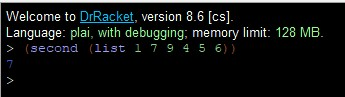
\includegraphics{ResultadoSecond.jpg}
\end{figure}

Los resultados de la función (append '(Bue) '(n semestre))
\begin{figure}[H]
    \centering
    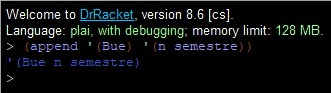
\includegraphics{ResultadoAppend.jpg}
\end{figure}

Nuestra propia implementación de append es esta:
\begin{figure}[H]
    \centering
    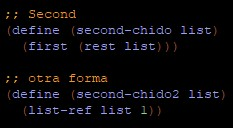
\includegraphics{SecondNuestro.jpg}
\end{figure}


Nuestra propia implementación de append es esta:
\begin{figure}[H]
    \centering
    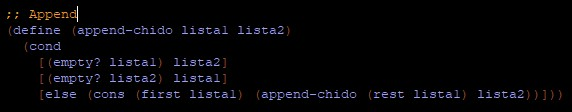
\includegraphics{AppendNuestro.jpg}
\end{figure}
